\documentclass[Main]{subfiles}
\begin{document}

\textbf{Optimization of implemented client}


- Ordering of goals and goals conflicting - maybe look for goals with most walls around (such as safe goals)

- Use partial plan as guideline for Heuristics

- Better subgoal decomposition

- "Better" back tracking

- Re-order goals?

% TODO re-read and fix
% social laws for Conflict, priority of agents, eg. agent has box, agent already started, agent closer to goal
- Multi-agent: Conflict handling
The current implementation lacks solid conflict handling when solving multi-agent levels. To make up for this, we propose to enhance the system with the methods described in \cite{pellier2007unified}. In this paper, an algorithm is described for solving multi agent problems where agents need to collaborate to solve a common goal. The algorithm uses me theologies from POP, HTN and a communication scheme between the agents to ensure the unified planning is consistent.

The algorithm works by initializing a POP with a set of open goals for the whole goal to be completed. Next, the algorithm will assign a complex action to each of the agents to solve a goal (footnote: complex action here refers to the higher level abstract actions which are used by HTN to refine into primitive actions, which in our case are for example moves or pushes). Hereafter, the algorithm will start to refine the complex actions into primitive actions. The agents take turn in refining one step of their complex actions into a primitive action, such that the agents are at the same time step in the unified execution. If a conflict arises in the plan, a threat is created which the agents will try to solve, first with a complex action, and next by an attempt to refine the complex action.
If a complex action fails and there is no way to solve the threat, then the algorithm must backtrack to the beginning of the failing complex action, and either try another refinement or attempt to refine one of the other complex actions first.
During the planning process the agents communicate about threats in the system, suggestions on how to repair a given threat, successfully completions of goals and refutations of other agents actions.
A threat can for example be that an agent is standing in the way of another agent, or a box is in the way of an agent and he need help to move it. A suggestion for a repair for a given threat, can for example be that an agent moves away from a given path. A refutation can be that an agent 0 refutes agent 1 to perform his action because agent 1 is moving to the same place as agent 0, in this case a solution could be to tell agent 1 to wait until agent 0 has passed.

\begin{figure}[h!]
	\centering
	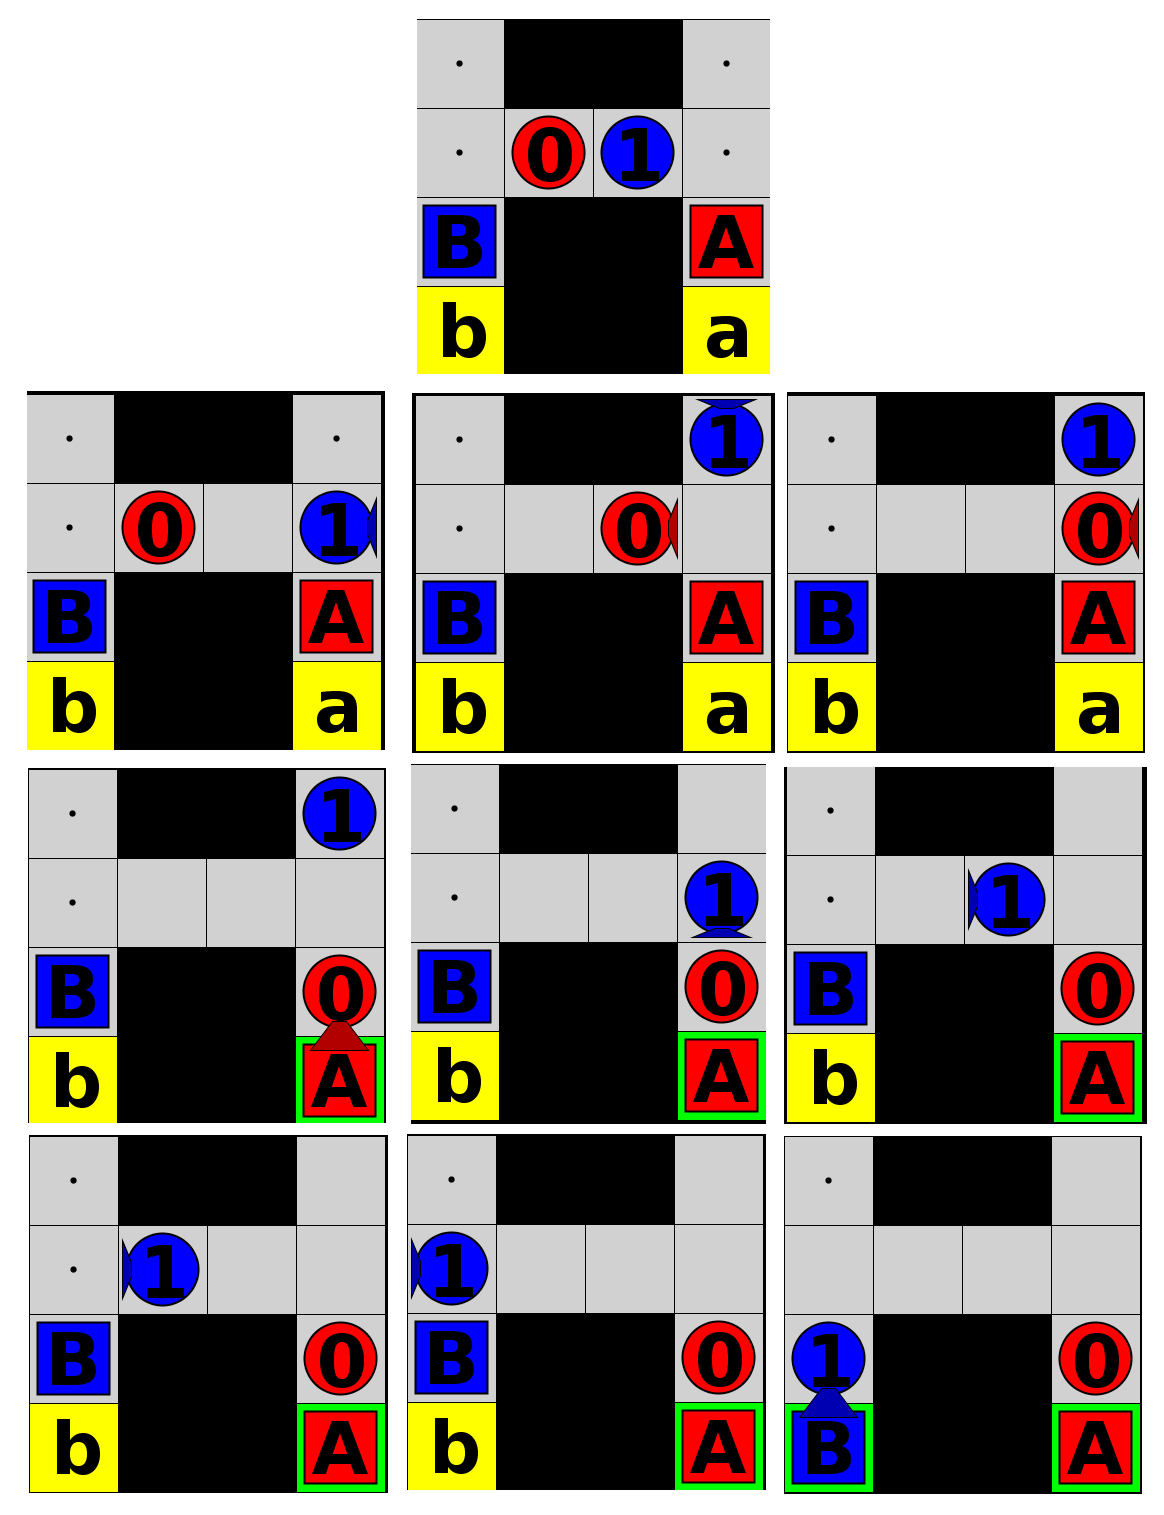
\includegraphics[width=0.3\textwidth]{plan_collab.png}
	\caption{Agent 0 needs to pass agent 1 in order to complete his goal, and vice versa}
	\label{fig:plan_collab}
\end{figure}

\begin{figure}[h!]
	\centering
	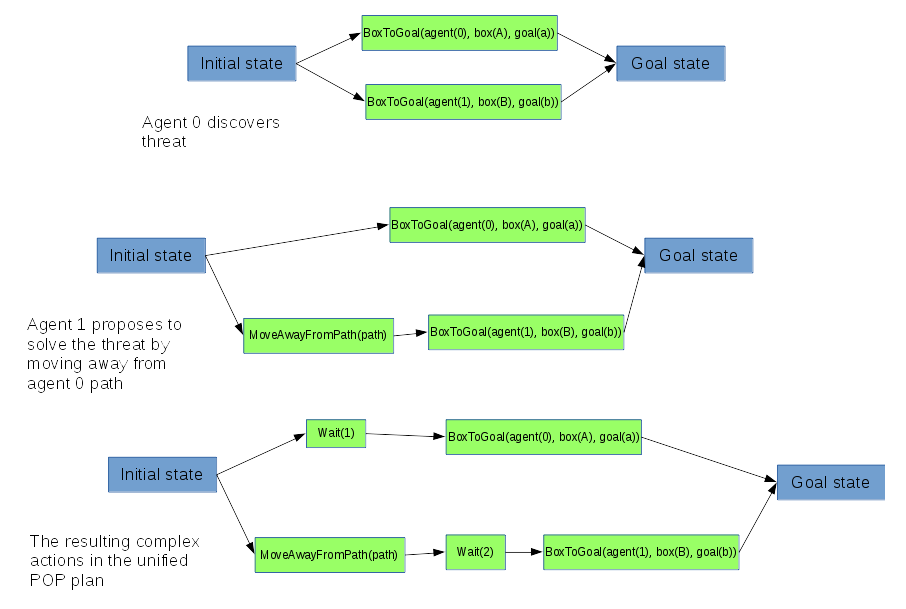
\includegraphics[width=0.5\textwidth]{unhtnpop.png}
	\caption{Example of a plan collaboration between agent 0 and 1 at complex action level}
	\label{fig:htn_collab}
\end{figure}


When agent 0 first tries to refine his complex action to complete goal a, he discovers that there is a conflict since agent 1 is standing in his way. Agent 0 can thus report failure, and open a new threat for getting a clear path to his goal. Next it is agent 1's turn to contribute to the plan, and he sees the threat, assign a complex action to be completed before his own goal completion complex action, and reports to all agents that he has done a repair to the unified plan. Next, agent 0 will attempt to refine his plan again, but will get a refutation from agent 1 since he is in the progress of moving out of the way, agent 1 can ask agent 0 to wait for one turn in this case. When agent 1 is out of the way, agent 0 can start refining his complex action properly and reach his goal. Agent 1 will attempt to refine his next complex action, which is to complete goal b, however agent 0 will refute his action and ask him to wait. This will continue until agent 0 is out of the way, and finally agent 1 can refine his complex action to solve goal b.
The process of the plan collaboration is visualized in Figure \ref{fig:htn_collab} and \ref{fig:plan_collab}.

- Communication

- Auction of 'unsolvable' or expensive goals \cite{VanderKrogt2005}
  - Cyclic dependencies 


- Pruning algorithm to limit branching factor [http://en.wikipedia.org/wiki/Pruning\_(decision\_trees)]
\todo[inline]{concurrency/parallel}

\end{document}
